\resizebox{\textwidth}{!}{
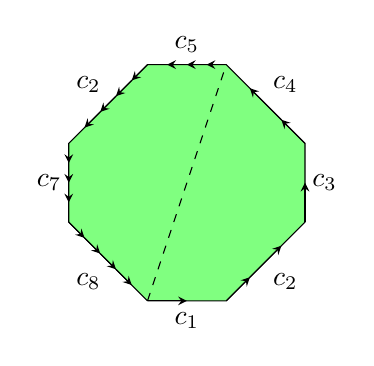
\begin{tikzpicture}
%Octógono
\draw[fill=green!50] (1,0) -- (2,0) -- (3,1) -- (3,2) -- (2,3) --
				(1,3) -- (0,2) -- (0,1) -- (1,0);

%La línea a través de la cual hacemos la suma conexa
\draw[dashed] (1,0) -- (2,3);

%Identificación de los lados
%c1
\draw[-stealth] (1,0) -- (1.5,0);
\draw (1.5,-.25) node {$c_1$};

%c2
\draw[-stealth] (2,0) -- (2.3,.3);
\draw[-stealth] (2.3,.3) -- (2.7,.7);
\draw (2.75,.25) node {$c_2$};

%c3
\draw[-stealth] (3,1) -- (3,1.5);
\draw (3.25,1.5) node {$c_3$};

%c4
\draw[-stealth] (3,2) -- (2.7,2.3);
\draw[-stealth] (2.7,2.3) -- (2.3,2.7);
\draw (2.75,2.75) node {$c_4$};

%c5
\draw[-stealth] (2,3) -- (1.75,3);
\draw[-stealth] (1.75,3) -- (1.5,3);
\draw[-stealth] (1.5,3) -- (1.25,3);
\draw (1.5,3.25) node {$c_5$};

%c6
\draw[-stealth] (1,3) -- (.8,2.8);
\draw[-stealth] (.8,2.8) -- (.6,2.6);
\draw[-stealth] (.6,2.6) -- (.4,2.4);
\draw[-stealth] (.4,2.4) -- (.2,2.2);
\draw (.25,2.75) node {$c_2$};

%c7
\draw[-stealth] (0,2) -- (0,1.75);
\draw[-stealth] (0,1.75) -- (0,1.5);
\draw[-stealth] (0,1.5) -- (0,1.25);
\draw (-.25,1.5) node {$c_7$};

%c8
\draw[-stealth] (0,1) -- (.2,.8);
\draw[-stealth] (.2,.8) -- (.4,.6);
\draw[-stealth] (.4,.6) -- (.6,.4);
\draw[-stealth] (.6,.4) -- (.8,.2);
\draw (.25,.25) node {$c_8$};
\end{tikzpicture}
}